\chapter{Diagramma di Dispersione - Velocità di Fase e Velocità di Gruppo}
Consideriamo ora un \textbf{generico modo} con \textbf{pulsazione di taglio} $\omega_t$ e valutiamo per $\omega > \omega_t$ la funzione:
\begin{equation*}
    \omega = \omega(\beta_z)
\end{equation*}
Che ci viene data in forma implicita da:
\begin{equation*}
    \beta^2_z = K^2 - K_t^2
\end{equation*}
Ovvero:
\begin{equation*}
    \beta^2_z = \frac{\omega^2}{c^2} - K_t^2
\end{equation*}
Dividendo ora entrambi i membri per $K^2_t$ otteniamo:
\begin{equation*}
    \frac{\omega^2}{K^2_t c^2}  - \frac{\beta^2_z}{K_t^2} = 1
\end{equation*}
E ricordando che $\omega_t = \frac{K_t}{\sqrt{\epsilon \mu}}$:
\begin{equation*}
    \frac{\omega^2}{\omega^2_t} - \frac{\beta^2_z}{K_t^2} = 1
\end{equation*}
Che non è altro che l'\textbf{equazione di un'iperbole}, i cui \textbf{asintoti} si calcolano facendo tendere $\beta_z \longrightarrow \infty$:
\begin{equation*}
\begin{aligned}
    &\frac{\omega^2}{\omega^2_t} - \frac{\beta^2_z}{K_t^2} = 1 \\
    &\frac{\omega^2}{\omega^2_t} = 1 + \frac{\beta^2_z}{K_t^2}\\
    &\text{Faccio tendere $\beta_z$ all'infinito}\\
    &\frac{\omega^2}{\omega^2_t} = \frac{\beta^2_z}{K_t^2}
\end{aligned}
\end{equation*}
Da cui ci possiamo ricavare l'equazione dell'\textbf{asintoto obliquo}:
\begin{equation*}
    \omega = \frac{\omega_t}{K_t} \beta_z = c \ \beta_z
\end{equation*}
\begin{center}
    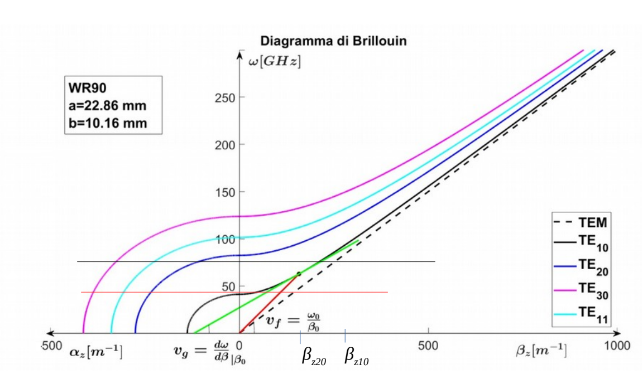
\includegraphics[width=\textwidth]{Images/figure45.png}
\end{center}
Consideriamo \textbf{un punto su un ramo di iperbole}, ad esempio quella nera, relativa al \textbf{modo fondamentale} $TE_{10}$, chiamandolo $(\omega_0, \beta_0)$ e tracciamo la \textbf{secante} a questo punto passante per l'origine (la retta rossa), che ha come equazione:
\begin{equation*}
    \omega = \nu_{fase} \beta_z
\end{equation*}
Dove il \textbf{coefficiente angolare} è:
\begin{equation*}
    \nu_{fase} = \frac{\omega_0}{\beta_0}
\end{equation*}
E che dovrebbe rappresentare la \textbf{velocità di propagazione di un segnale di pulsazione} $\omega_0$ sul \textbf{modo fondamentale}.\\ 
Tuttavia come si evince dal disegno $\nu_f > c$ ma questo è \textbf{impossibile}!!\\ \\
Per questo la \textbf{vera velocità} con cui viene trasportata l'informazione non è $\nu_{fase}$ ma:
\begin{equation*}
    \nu_{gruppo} = \frac{d \omega}{d \beta_z}\left(\omega_0 \right)
\end{equation*}
Che non è altro che il \textbf{coefficiente angolare della retta tangente al punto} (linea verde) che è \textbf{più piccolo della velocità della luce}.\\ \\
Ritorniamo ora a questa relazione:
\begin{equation*}
    \frac{\omega^2}{\omega^2_t} = 1 + \frac{K^2_z}{K_t^2}
\end{equation*}
\begin{equation*}
    \omega^2 = \omega^2_t + \omega^2_t \frac{K^2_z}{K_t^2}
\end{equation*}
\begin{equation*}
    \omega = \sqrt{\omega^2_t + c^2 K^2_z}
\end{equation*}
Ed ora differenziamola:
\begin{equation*}
    \frac{d \omega}{d K_z} = \frac{1}{2} \frac{1}{\underbrace{\sqrt{\omega^2_t + c^2 K^2_z}}_{\omega}} 2 c^2 K_z = \frac{c^2 K_z}{\omega} = \nu_{gruppo} = c^2 \cdot \frac{1}{\nu_f}
\end{equation*}